% Springer Nature article template, version 3.1 (December 2024)
% Target journal: Neural Processing Letters
\documentclass[pdflatex,sn-mathphys-num]{sn-jnl}

\usepackage{graphicx}
\usepackage{amsmath,amssymb,amsfonts,amsthm,bm}
\usepackage{booktabs}
\usepackage{array}
\usepackage{xurl}

\theoremstyle{thmstyleone}
\newtheorem{proposition}{Proposition}

\newcommand{\R}{\mathbb{R}}
\newcommand{\M}{\bm{M}}
\newcommand{\Q}{\bm{Q}}
\newcommand{\U}{\bm{U}}
\newcommand{\kvec}{\bm{k}}
\newcommand{\qvec}{\bm{q}}
\newcommand{\vvec}{\bm{v}}
\newcommand{\evec}{\bm{e}}
\newcommand{\avec}{\bm{a}}
\newcommand{\zvec}{\bm{z}}
\newcommand{\diag}{\operatorname{diag}}
\newcommand{\norm}[1]{\lVert#1\rVert}
\newcommand{\QDDD}{\ensuremath{\mathrm{QD}^{3}}}

\begin{document}

\title[Query Dual Dynamics Delta]{Query Dual Dynamics Delta: Read-Driven Modulation of Delta-Rule Writes in Fixed-Capacity Fast-Weight Memory}

\author*[1]{\fnm{Dian} \sur{Yu}}\email{dian.yu2@student.unsw.edu.au}
\author[1]{\fnm{Haoyu} \sur{Yang}}\email{z5575389@ad.unsw.edu.au}
\affil*[1]{\orgname{University of New South Wales},
  \orgaddress{\city{Sydney}, \postcode{2052}, \state{NSW}, \country{Australia}}}

\abstract{A fixed-capacity fast-weight memory is normally updated from the stream being written, although its usefulness is determined by a possibly different stream of future reads. This paper introduces Query Dual Dynamics Delta (\QDDD), an online operator that turns past queries into causal guidance for subsequent Delta writes. One state stores key--value associations; a second, low-rank state follows the dominant directions and energy of the query stream. Their only coupling is an interpretable scalar: the estimated historical query heat of the incoming write key. This heat increases the residual-correction rate, while a hard cap preserves the non-expansive single-address behavior of the normalized Delta rule. The construction adds $O(d_k r)$ state, is constant in sequence length, and recovers ordinary Delta exactly when query modulation is disabled. We evaluate the operator without end-to-end training so that memory behavior is measured directly. Hyperparameters are selected on eight validation seeds and frozen for 16 paired test seeds. \QDDD\ reduces normalized recall error by 31.0\% on a concentrated spatial field, 18.7\% on a source-token workload, 32.1\% on a module-import graph, and 2.62\% on held-out WikiText-2 token sequences. An estimator- and capacity-matched write-trace control establishes that the additional information comes from reads rather than extra state. Uniform-query, moving-hotspot, source, and rank controls further delimit the mechanism.}

\keywords{fast-weight memory, Delta rule, linear attention, associative memory, workload adaptation, online subspace learning}

\maketitle

\section{Introduction}\label{sec:intro}

A compact memory is valuable precisely because it does not grow with the history it summarizes. The same constraint also creates competition: after sufficiently many key--value pairs have been written, improving one association can disturb another. Delta-style fast weights address part of this problem by writing only the residual that is still missing at the current key~\cite{widrow1960,schlag2021}. They answer a local question---\emph{what is wrong at this write address?}---but not the allocation question---\emph{which addresses will matter when this memory is read?}

That distinction is immaterial when writes and reads have the same distribution. It becomes important for a long-running service, agent, map, or compressed sequence state in which the stored population is broad but the workload is concentrated. A small set of entities may be queried repeatedly even though every entity is written with comparable frequency. Write counts cannot reveal this demand. Recency cannot reveal it either. The read events themselves carry the missing signal.

We therefore treat a query as more than a transient probe. In Query Dual Dynamics Delta (\QDDD), reads learn a compact workload state, writes learn the key--value map, and a single non-negative heat value connects them. The core innovation is this causal cross-event allocation: accumulated read geometry controls the rate of \emph{later} residual writes in a continuous, fixed-capacity memory. It neither performs an instantaneous query correction nor evicts discrete cached tokens. The two independently evolving states give the method its name.

The design follows four principles: only earlier reads may affect a write; cold-start behavior must remain ordinary Delta; the workload state must be much smaller than the memory it guides; and prioritization must remain inside the normalized Delta stability interval. These requirements lead directly to a causal low-rank query trace and a clipped effective write rate.

We study the operator separately from an end-to-end model so that its central hypothesis is directly testable: given identical writes, capacity, and evaluation samples, does read history improve later recall? The study uses a smooth two-dimensional field, two real-data-derived controlled workloads, and held-out WikiText-2 sequences~\cite{merity2016wikitext}. Its decisive baseline matches the low-rank estimator, state size, update count, normalization, and tuning budget, but learns from write keys instead of query keys.

The contributions are:
\begin{itemize}
  \item a causal read-driven Delta operator that uses accumulated query geometry to allocate corrective write rate;
  \item a low-rank query trace whose heat has a direct interpretation as discounted squared query--key alignment, with constant state in the stream length;
  \item a clipped update with exact reduction to ordinary Delta and a simple non-expansion guarantee at the written address; and
  \item a paired, validation-separated study that includes an estimator-matched source control, full-moment and weighted-linear references, rank and source ablations, uniform-query controls, and a changing workload.
\end{itemize}

\section{Related work}\label{sec:related}

\subsection{Fast weights and Delta-based linear attention}

Fast weights are parameters that change on the time scale of a sequence and store temporary associations~\cite{schmidhuber1992,ba2016}. Kernelized linear attention can be written as a recurrent matrix update with state independent of sequence length~\cite{katharopoulos2020}. The fast-weight-programming view makes the connection explicit: keys and values form programming instructions for a finite associative matrix~\cite{schlag2021}. Purely additive writing accumulates interference, whereas the Delta rule first subtracts the value already predicted at the current key and writes only the residual. Parallel DeltaNet later supplied a sequence-parallel implementation and demonstrated the rule at language-model scale~\cite{yang2024parallel}.

Recent work has improved how the current token edits this matrix. Gated DeltaNet combines targeted Delta correction with a forgetting gate~\cite{yang2025gated}; Gated DeltaNet-2 separates channel-wise erase and write gates~\cite{hatamizadeh2026gdn2}; and DeltaProduct applies several Delta steps per token, increasing the rank and expressivity of the transition~\cite{siems2025deltaproduct}. These mechanisms decide how to edit from the current input and learned gates. \QDDD\ addresses a different variable: the empirical distribution of earlier reads.

The closest query-aware operators also use the current query more directly. Q-Delta mixes current key- and query-based prediction errors in one state transition~\cite{park2026qdelta}. Query-derived Erase Direction introduces a second, current-query erase direction to remove interference that a key-directed edit cannot reach~\cite{gupta2026qed}. Both are instantaneous query--write couplings at a sequence position. \QDDD\ instead accumulates a query second-moment surrogate over many read events and uses it to price future writes. The distinction is operational: a current query answers \emph{what should be corrected now?}; a query history estimates \emph{where future correction effort is likely to be useful?}

\begin{table}[t]
\caption{Position of \QDDD\ among memory-management mechanisms. ``Current'' denotes information at the present sequence position; ``history'' denotes a separately accumulated statistic. Citations and fuller distinctions are given in Sect.~\ref{sec:related}.}
\label{tab:related}
\centering
\small
\setlength{\tabcolsep}{3pt}
\begin{tabular}{@{}p{0.19\textwidth}p{0.18\textwidth}p{0.24\textwidth}p{0.31\textwidth}@{}}
\toprule
Method family & Guidance & What changes & Difference from \QDDD \\
\midrule
DeltaNet & current key and residual & one corrective write & no read-history model \\
Gated DeltaNet & current-token gates & forgetting and/or writing & learned current-token control \\
DeltaProduct & current-token residuals & multiple Delta steps & increases transition rank \\
Q-Delta / QED & current query & correction or erase direction & instantaneous query-aware edit \\
H$_2$O / SnapKV & attention observations & stored token positions & evicts from a discrete KV cache \\
\QDDD\ (ours) & query history & future residual-write rate & cumulative continuous-state allocation \\
\bottomrule
\end{tabular}
\end{table}

\subsection{Access-aware retention and online subspaces}

Read frequency has also been exploited in explicit key--value caches. H$_2$O retains attention heavy hitters together with recent tokens~\cite{zhang2023h2o}, while SnapKV estimates important prompt positions from an observation window and compresses the discrete cache~\cite{li2024snapkv}. Those methods choose which token records remain available. A fast-weight matrix has no token list to evict after associations have been superposed, so access information must act through the continuous write rule instead. This is the gap addressed here.

The low-rank query state is updated by an Oja-type subspace rule~\cite{oja1982}. Oja's algorithm is a standard streaming route to principal directions, with established multi-component guarantees~\cite{huang2021oja}. OjaKV recently used online Oja adaptation for low-rank compression of an explicit KV cache~\cite{zhu2025ojakv}. In \QDDD, no cached value is projected or discarded by this subspace. It approximates only the query workload and produces a scalar importance signal for the separate value memory.

At a statistical level, the motivation is related to covariate-shift correction: when training and test inputs differ, importance weighting aligns the fitted objective with the test distribution~\cite{sugiyama2007}. Exact importance weighting requires a density ratio. \QDDD\ neither estimates nor claims to recover that ratio. It uses a cheaper geometric proxy---discounted query energy near a key---that can be maintained online when only read addresses, not read-time target values, are available.

\section{Problem formulation}\label{sec:problem}

Consider two interleaved event streams. A write event provides a key--value pair $(\kvec_t,\vvec_t)$ with $\kvec_t\in\R^{d_k}$ and $\vvec_t\in\R^{d_v}$. A query event provides an address $\qvec_j\in\R^{d_k}$. The indices $t$ and $j$ count writes and queries separately; $j(t)$ denotes the number of queries observed before write $t$. All keys and queries are normalized to unit Euclidean norm in our experiments.

The fixed-capacity value state is $\M_t\in\R^{d_v\times d_k}$. A query is answered by
\begin{equation}
 \widehat{\vvec}(\qvec_j)=\M_t\qvec_j.
 \label{eq:read}
\end{equation}
For a write, ordinary Delta first computes the current prediction and residual,
\begin{equation}
 \widehat{\vvec}_t=\M_{t-1}\kvec_t,
 \qquad
 \evec_t=\vvec_t-\widehat{\vvec}_t,
 \label{eq:residual}
\end{equation}
then performs the rank-one correction
\begin{equation}
 \M_t=\M_{t-1}+\eta\evec_t\kvec_t^{\mathsf T},
 \label{eq:plain-delta}
\end{equation}
where $\eta\geq0$ is the write rate. Because $\norm{\kvec_t}=1$, Eq.~\eqref{eq:plain-delta} is a stochastic-gradient step on $\tfrac12\norm{\vvec_t-\M\kvec_t}^2$.

Let $p_w$ denote the distribution of associations presented for writing and $p_q$ the workload under which recall is evaluated. The desired linear state minimizes
\begin{equation}
 \mathcal{L}_q(\M)=\frac12\,\mathbb{E}_{(\kvec,\vvec)\sim p_q}
 \left[\norm{\vvec-\M\kvec}^{2}\right].
 \label{eq:query-risk}
\end{equation}
Plain Delta samples gradients under $p_w$. If $p_q\neq p_w$, even a well-tuned write process spends its updates according to the population presented, not the population later requested. An exact correction would multiply each gradient by $p_q(\kvec)/p_w(\kvec)$, but estimating a high-dimensional density ratio online is a substantially different problem. We seek a local signal that is available from queries alone and cheap enough to attach to every Delta memory.

\section{Query Dual Dynamics Delta}\label{sec:method}

\subsection{The full query heat}

Suppose first that storing a full $d_k\times d_k$ query statistic is affordable. After query $j$, define the exponentially weighted, uncentered second moment
\begin{equation}
 \Q_j=\lambda\Q_{j-1}+\qvec_j\qvec_j^{\mathsf T},
 \qquad 0<\lambda\leq1.
 \label{eq:full-trace}
\end{equation}
For any candidate write key $\kvec$, its unnormalized query heat is
\begin{equation}
 \bar h_j(\kvec)=\kvec^{\mathsf T}\Q_j\kvec
 =\sum_{\ell=1}^{j}\lambda^{j-\ell}(\qvec_{\ell}^{\mathsf T}\kvec)^2.
 \label{eq:heat-identity}
\end{equation}
Equation~\eqref{eq:heat-identity} gives the central quantity a direct reading. Every earlier query votes for a new write in proportion to squared alignment in key space; the square makes the vote independent of sign, and $\lambda$ determines how quickly old demand is forgotten. A key receives high heat when it lies in directions that have repeatedly been queried. No queried target value is required.

The full trace is useful as a reference, but its $d_k^2$ state can rival or exceed the memory being guided. \QDDD\ therefore maintains a low-rank surrogate.

\subsection{Low-rank query dynamics}

Let $\U_j=[\bm u_{j,1},\ldots,\bm u_{j,r}]\in\R^{d_k\times r}$ contain $r\ll d_k$ adaptive directions and let $\avec_j\in\R_+^r$ store their discounted energies. When query $\qvec_j$ arrives, we first project it into the current subspace,
\begin{equation}
 \zvec_j=\U_{j-1}^{\mathsf T}\qvec_j.
 \label{eq:projection}
\end{equation}
The residual $\qvec_j-\U_{j-1}\zvec_j$ is the part not reconstructed by that subspace. An Oja-type step rotates the directions toward this missing component:
\begin{equation}
 \U_j=\U_{j-1}+\eta_u
 \bigl(\qvec_j-\U_{j-1}\zvec_j\bigr)\zvec_j^{\mathsf T},
 \label{eq:oja}
\end{equation}
where $\eta_u$ is the subspace rate. At the same event, projected energy is accumulated as
\begin{equation}
 \avec_j=\lambda\avec_{j-1}+\zvec_j\odot\zvec_j.
 \label{eq:energy}
\end{equation}
Here $\odot$ denotes elementwise multiplication. Equations~\eqref{eq:oja} and \eqref{eq:energy} have complementary roles: $\U_j$ tracks \emph{which directions} queries occupy, while $\avec_j$ tracks \emph{how much demand} lies along each direction. The factorized moment surrogate is $\U_j\diag(\avec_j)\U_j^{\mathsf T}$, so the heat assigned to an incoming write key is
\begin{equation}
 \bar h_j(\kvec_t)=
 \sum_{i=1}^{r}a_{j,i}(\bm u_{j,i}^{\mathsf T}\kvec_t)^2.
 \label{eq:lowrank-heat}
\end{equation}

The magnitude of Eq.~\eqref{eq:lowrank-heat} depends on query count and geometry. To keep $\beta$ interpretable across streams, we maintain one causal scale
\begin{equation}
 s_j=\max\!\left\{s_{j-1},
 \sum_{i=1}^{r}a_{j,i}(\bm u_{j,i}^{\mathsf T}\qvec_j)^2,\epsilon\right\},
 \qquad
 h_j(\kvec)=\frac{\bar h_j(\kvec)}{s_j},
 \label{eq:normalization}
\end{equation}
with a small numerical $\epsilon>0$. This maximum-observed scale is a normalization device, not an additional learned parameter. It uses only information available at query $j$.

\subsection{Read-driven rate and memory update}

For write $t$, \QDDD\ uses the most recent query state $j(t)$ and sets
\begin{equation}
 \widetilde\eta_t=min\left\{
 \eta\bigl[1+\beta h_{j(t)}(\kvec_t)\bigr],\ c\right\},
 \qquad \beta\geq0,
 \label{eq:rate}
\end{equation}
followed by
\begin{equation}
 \M_t=\M_{t-1}+\widetilde\eta_t
 \bigl(\vvec_t-\M_{t-1}\kvec_t\bigr)\kvec_t^{\mathsf T}.
 \label{eq:qddd}
\end{equation}
The constant $1$ in Eq.~\eqref{eq:rate} matters. It retains the ordinary Delta update during cold start and for directions with no query evidence. The coefficient $\beta$ controls only the additional effort assigned by the workload trace. Setting $\beta=0$ makes $\widetilde\eta_t=\eta$ whenever $\eta\leq c$, so Eq.~\eqref{eq:qddd} is exactly Eq.~\eqref{eq:plain-delta}; this equality is also tested numerically in both implementations.

The cap $c$ is a safeguard for the residual correction, not a cosmetic clamp. For unit-norm keys, the following property is immediate.

\begin{proposition}[Written-address non-expansion]\label{prop:stable}
Let $\norm{\kvec_t}=1$ and $0\leq\widetilde\eta_t\leq2$. If $\evec_t$ is the pre-update residual in Eq.~\eqref{eq:residual}, the residual at the same key after Eq.~\eqref{eq:qddd} is
\begin{equation}
 \evec_t^{+}=(1-\widetilde\eta_t)\evec_t,
\end{equation}
and therefore $\norm{\evec_t^{+}}\leq\norm{\evec_t}$.
\end{proposition}

\begin{proof}
Multiplying Eq.~\eqref{eq:qddd} by $\kvec_t$ and using $\kvec_t^{\mathsf T}\kvec_t=1$ gives
$\M_t\kvec_t=\M_{t-1}\kvec_t+\widetilde\eta_t\evec_t$.
Subtracting from $\vvec_t$ yields the stated identity. The norm inequality follows from $|1-\widetilde\eta_t|\leq1$ on $[0,2]$.
\end{proof}

We use $c=1.9$, leaving a margin below the endpoint. Proposition~\ref{prop:stable} is local to the written address; as with every shared fast-weight matrix, interference at other keys is still possible. It nevertheless explains why workload amplification is clipped before entering the Delta rule.

Figure~\ref{fig:architecture} summarizes the complete event flow. Query events update $(\U,\avec,s)$ and are answered from $\M$ without directly changing it. Write events consult the frozen query state to update $\M$ and do not train the query trace. This separation prevents write frequency from leaking into the quantity meant to represent read demand.

\begin{figure}[t]
\centering

\includegraphics[width=\textwidth]{figures/Fig1_qd3_architecture.pdf}
\caption{Query Dual Dynamics Delta. A query updates the low-rank workload state and is answered by the fixed-capacity value memory. A later write is scored against the accumulated query directions; the normalized heat modulates the ordinary residual Delta correction. The two states evolve on different event types and communicate only through the scalar heat. Setting $\beta=0$ exactly recovers Plain Delta.}
\label{fig:architecture}
\end{figure}

\subsection{State and computational cost}

The value memory contains $d_vd_k$ scalars. \QDDD\ adds $d_kr+r+1$ scalars for $\U$, $\avec$, and $s$, independent of the number of events. Its additional state fraction is therefore
\begin{equation}
 \frac{d_kr+r+1}{d_vd_k}\approx\frac{r}{d_v}
 \quad\text{when }d_k,d_v\text{ are not small}.
\end{equation}
A query needs $O(d_vd_k)$ work for recall and $O(d_kr)$ for the trace update. A write retains the $O(d_vd_k)$ Delta prediction and outer product and adds an $O(d_kr)$ heat calculation. The full-trace reference adds $d_k^2$ state and $O(d_k^2)$ trace work. The low-rank construction is consequently most attractive when $r\ll\min(d_k,d_v)$.

\section{Experimental design}\label{sec:experiments}

\subsection{Tasks and evaluation metric}

The experiments isolate memory quality: there is no learned encoder, classifier, or end-to-end task head. This avoids attributing to the write rule gains that could instead come from additional model training.

\subsubsection{Synthetic spatial field}
Write locations are sampled uniformly from $[0,1]^2$. A fixed 64-dimensional random Fourier map produces unit keys, and an eight-dimensional smooth harmonic field produces values with additive Gaussian noise of standard deviation $0.05$. Query and evaluation locations are sampled independently. In the concentrated condition they come from two Gaussian hotspots; in the uniform condition they cover the square uniformly. A moving-hotspot condition switches to a disjoint pair halfway through the query stream. Each run has 3,000 writes and 5,000 evaluation samples. This controlled source is included to expose the mechanism under known independent distributions, rather than as an application benchmark.

\subsubsection{Real-data-derived controlled workloads}
Two structurally different streams are constructed from source-code text. The token workload contains 3,000 identifiers: short-window co-occurrence features are reduced to $d_k=128$ keys, long-window profiles give $d_v=64$ values, and observed token counts define read frequency. The module-import graph contains 578 modules: co-import structure gives $d_k=24$ keys and $d_v=48$ values, while import counts define the read distribution. Writes traverse every item in random order for three and six passes, respectively. These tasks retain real heavy-tailed workloads and geometry while allowing exact control of the read distribution. They are used for mechanism confirmation, not presented as end-to-end software applications.

\subsubsection{WikiText-2 held-out token sequence}
WikiText-2 is a public corpus of curated Wikipedia articles~\cite{merity2016wikitext}. The training split fixes a 3,000-word vocabulary and builds a unit-normalized 256-dimensional short-window co-occurrence key for each word; normalized 64-dimensional long-window context profiles are the stored values. The write stream makes two independently shuffled passes over these 3,000 associations. Query events and evaluation items, however, come from a contiguous, disjoint window of the held-out validation or test token sequence: a query prefix is immediately followed by the scored portion. A shuffled-query control keeps the same query multiset and changes only its order. The prepared vocabulary covers 84.1\% of held-out test tokens, and the most frequent 10\% of vocabulary items account for 72.5\% of covered test occurrences. Each run evaluates 3,000 held-out tokens.

For $N$ evaluation associations $(\kvec_n,\vvec_n)$, lower normalized root mean squared error (NRMSE) is better:
\begin{equation}
 \operatorname{NRMSE}=
 \frac{\sqrt{N^{-1}\sum_{n=1}^{N}\norm{\M\kvec_n-\vvec_n}^{2}}}
 {\sqrt{N^{-1}\sum_{n=1}^{N}\norm{\vvec_n}^{2}}}.
 \label{eq:nrmse}
\end{equation}
Sampling evaluation items from the query workload makes Eq.~\eqref{eq:nrmse} a Monte Carlo estimate of Eq.~\eqref{eq:query-risk}, normalized for comparability.

\subsection{Baselines and controls}

Plain Delta is Eq.~\eqref{eq:plain-delta}. The main source control, \emph{Write Trace}, is deliberately matched to \QDDD: it uses the same Oja update, rank choices, energy decay, heat normalization, number of trace events, rate equation, and validation budget, but supplies the contemporaneous write key to Eqs.~\eqref{eq:projection}--\eqref{eq:energy}. A difference between these two methods can therefore be attributed to the information source rather than additional state or computation.

The \emph{Full Query Trace} uses Eq.~\eqref{eq:full-trace} without low-rank approximation. The \emph{Stationary Query Moment} receives the true stationary query second moment and uses the same scalar gain; it is an offline reference, not an upper bound. The \emph{Weighted Linear} reference solves ridge-stabilized least squares under the evaluation weights. It is optimal only within a stationary linear-map class and is not a bound on arbitrary memory systems.

Mechanism ablations replace the learned low-rank trace with a coordinate-wise diagonal moment, the most recent query alone, or a fixed random rank-four subspace. Rank is swept over $r\in\{1,2,4,8,16\}$. Uniform queries test the case in which the query source carries no distributional preference beyond broad coverage. Query-frequency power $\alpha\in\{0,0.25,0.5,0.75,1,1.25\}$ continuously changes the controlled discrete workloads from uniform ($\alpha=0$) to and beyond their observed skew ($\alpha=1$).

\subsection{Selection, pairing, and implementation checks}

Pilot seeds inspected during development are excluded. For the synthetic and controlled workloads, eight new validation seeds (2001--2008) select hyperparameters and 16 locked test seeds (10001--10016) are evaluated once. WikiText-2 uses validation seeds 4001--4008 and disjoint test seeds 30001--30016. Every method within a seed receives the same write order, query sequence, and evaluation samples. Each test seed occupies a disjoint block of the held-out token sequence before its contiguous window is selected.

The main search uses $\eta\in\{0.02,0.05,0.1,0.2,0.4\}$, $\beta\in\{1,3,10,30,100\}$, and $r\in\{2,4,8\}$ for low-rank methods. WikiText-2 uses $\eta\in\{0.02,0.05,0.1\}$, $\beta\in\{1,3,10,30\}$, and $r\in\{1,2,4\}$. Each method is tuned separately on validation NRMSE. Fixed operator settings are $\eta_u=0.05$, $\lambda=0.999$, $c=1.9$, and one query event per three writes.

We report test means, sample standard deviations, and paired differences with two-sided 95\% Student-$t$ confidence intervals over 16 seeds. The pre-specified primary comparisons are \QDDD\ versus Plain Delta and versus Write Trace; full-trace comparisons are secondary. Complete validation grids, selected settings, per-seed observations, manifests, and file hashes accompany the manuscript. Unit tests cover finite outputs, batched/individual agreement, deterministic replay, exact $\beta=0$ reduction, source isolation, and agreement among NumPy, Torch, and CUDA implementations to within $2\times10^{-4}$.

\section{Results}\label{sec:results}

\subsection{Concentrated and held-out workloads}

Table~\ref{tab:main} reports the four principal non-uniform workloads. On the controlled spatial field, \QDDD\ lowers NRMSE from $0.7305$ to $0.5040$, a 31.0\% reduction. Write Trace does not improve Plain Delta, whereas the low-rank query trace is statistically indistinguishable from the full online query moment (paired difference $-0.0007$, 95\% CI $[-0.0042,0.0029]$). Thus, the spatial gain is neither a general consequence of adaptive rates nor dependent on storing a dense moment.

The two real-data-derived workloads reproduce the effect across text statistics and graph structure. \QDDD\ reduces error by 18.7\% on token profiles and 32.1\% on the module-import graph. Write frequency is informative here: Write Trace already obtains reductions of 16.8\% and 27.8\%. The remaining paired improvements of \QDDD\ are nevertheless consistent: the \QDDD--Write Trace differences are $-0.0144$ (95\% CI $[-0.0216,-0.0071]$; 14/16 wins) and $-0.0391$ (95\% CI $[-0.0460,-0.0321]$; 16/16 wins), respectively. Reads therefore supply information beyond a strong frequency-based baseline.

On held-out WikiText-2 sequences, the effect is smaller but remains paired and repeatable. \QDDD\ reduces NRMSE by 2.62\% relative to Plain Delta and by 1.42\% relative to Write Trace; the paired difference is $-0.0024$ (95\% CI $[-0.0034,-0.0014]$; 14/16 wins). Its mean differs from the full trace by only $8.6\times10^{-5}$, with a confidence interval spanning zero. Shuffling the order of the same query multiset changes \QDDD's gain from 2.62\% to 2.46\%; frequency and key geometry, rather than a fragile local token ordering effect, account for most of the result.

\begin{table}[t]
\caption{Blind-test NRMSE on non-uniform workloads, reported as mean (sample standard deviation) over 16 paired seeds. Gain is the relative reduction of \QDDD\ from Plain Delta. Paired \QDDD--Write Trace confidence intervals are reported in the surrounding text.}
\label{tab:main}
\centering
\scriptsize
\setlength{\tabcolsep}{3pt}
\begin{tabular}{@{}lccccc@{}}
\toprule
Workload & Plain & Write trace & \QDDD & Full trace & Gain (\%) \\
\midrule
Spatial, concentrated & $.7305$ ($.0450$) & $.7347$ ($.0534$) & $\bm{.5040}$ ($.0455$) & $.5047$ ($.0467$) & $31.01$ \\
Source-token profiles & $.7718$ ($.0391$) & $.6421$ ($.0243$) & $\bm{.6278}$ ($.0164$) & $.6143$ ($.0096$) & $18.66$ \\
Module-import graph & $.8923$ ($.0219$) & $.6447$ ($.0282$) & $\bm{.6056}$ ($.0190$) & $.6035$ ($.0171$) & $32.13$ \\
WikiText-2, ordered & $.1719$ ($.0157$) & $.1698$ ($.0160$) & $\bm{.1674}$ ($.0147$) & $.1673$ ($.0148$) & $2.62$ \\
\bottomrule
\end{tabular}
\end{table}

Figure~\ref{fig:main-results} places the central positive conditions beside their uniform controls. Under uniform spatial queries, \QDDD\ and Write Trace are indistinguishable (paired difference $-0.00021$, 95\% CI $[-0.00084,0.00042]$), and both are slightly worse than Plain Delta. In the uniform WikiText-2 workload, both adaptive low-rank methods improve Plain Delta by about 1.2\%, but their difference is only $3.1\times10^{-5}$ NRMSE. The same source equality appears on uniform token and import workloads: the paired \QDDD--Write Trace confidence intervals both include zero. The relevant boundary is therefore precise: when queries carry no extra allocation information, the query trace loses its advantage over its matched write-derived counterpart. Our claim concerns workload-aware allocation, not universal improvement under identical event distributions.

\begin{figure}[t]
\centering
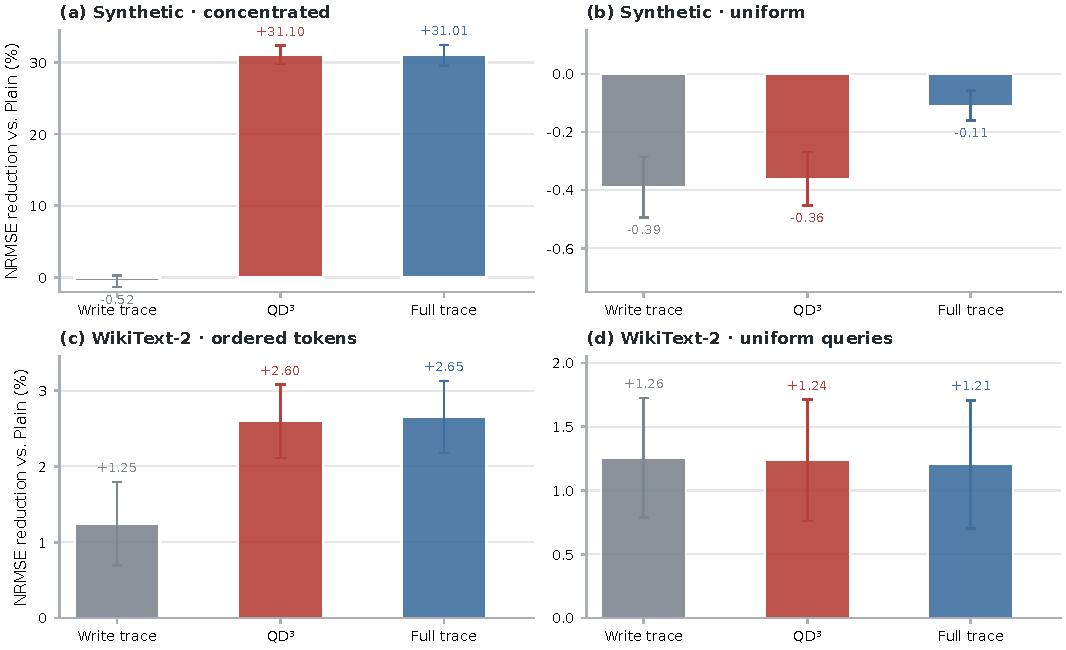
\includegraphics[width=0.96\linewidth]{figures/Fig2_main_results.pdf}
\caption{Blind-test NRMSE reduction relative to Plain Delta (mean and paired 95\% confidence interval; 16 seeds; each panel has its own labeled vertical scale). On the controlled spatial field, query-derived traces improve concentrated-query recall while the matched write trace does not; their distinction disappears under uniform queries. On WikiText-2, contiguous held-out queries give \QDDD\ a 2.62\% reduction, whereas \QDDD\ and Write Trace are nearly identical under uniform queries. Lower NRMSE is better.}
\label{fig:main-results}
\end{figure}

\subsection{Where the gain comes from}

The query-skew sweep in Fig.~\ref{fig:mechanism}a tests the proposed cause continuously rather than only at two endpoints. At $\alpha=0$, \QDDD\ has no measurable advantage over Write Trace. As read demand becomes more concentrated, the advantage grows monotonically to 2.90\% on token profiles and 7.20\% on the import graph at $\alpha=1.25$. This is the pattern expected if the second state measures workload mismatch: changing the query distribution changes the value of query history while leaving the write population fixed.

Figure~\ref{fig:mechanism}b and Table~\ref{tab:ablation} examine representation. A fixed random rank-four subspace is ineffective, so state count alone is not sufficient. A diagonal trace works when demand is aligned with input coordinates but fails on the rotated spatial features. The most recent query captures some locality, yet accumulated geometry is consistently stronger on the spatial task. Learned ranks between one and four recover essentially all of the full-trace benefit on the two real-data-derived workloads; the spatial field needs four directions for its best test mean. Larger rank is not automatically better because validation chooses one global $(\eta,\beta)$ and finite-stream subspace estimates become noisier. The result supports compression of the workload statistic, not a claim that one rank is universal.

\begin{figure}[t]
\centering
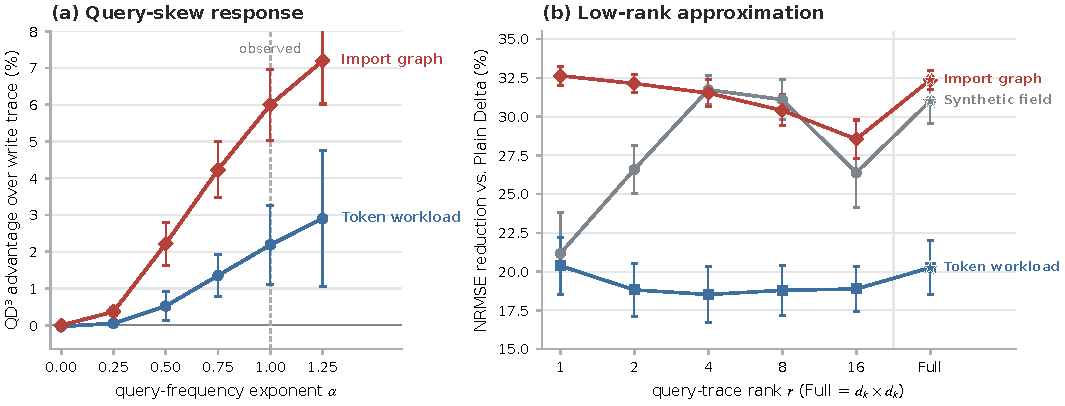
\includegraphics[width=0.96\linewidth]{figures/Fig3_mechanism_and_ablation.pdf}
\caption{Mechanism tests on blind seeds. (a) The additional NRMSE reduction of \QDDD\ over the estimator- and capacity-matched Write Trace grows with the query-frequency exponent and begins near zero for uniform queries. (b) A small adaptive query subspace recovers the full online second-moment result; optimal rank is task dependent and selected only on validation seeds.}
\label{fig:mechanism}
\end{figure}

\begin{table}[t]
\caption{Ablation results as percentage NRMSE reduction from Plain Delta. ``Random'' uses a fixed random rank-four subspace; ``best low rank'' reports the best tested rank by blind-test mean for interpretation, while all headline ranks in Table~\ref{tab:main} were selected on validation data.}
\label{tab:ablation}
\centering
\small
\begin{tabular}{lrrrrr}
\toprule
Workload & Diagonal & Last query & Random & Best low rank & Full trace \\
\midrule
Spatial, concentrated & $-0.82$ & $16.09$ & $-0.64$ & $31.73$ ($r=4$) & $30.91$ \\
Source-token profiles & $18.30$ & $20.12$ & $1.70$ & $20.53$ ($r=1$) & $20.40$ \\
Module-import graph & $27.50$ & $30.71$ & $3.00$ & $32.65$ ($r=1$) & $32.37$ \\
\bottomrule
\end{tabular}
\end{table}

\subsection{Changing demand}

The moving-hotspot experiment changes the query center halfway through the stream and evaluates the final region. Plain Delta obtains $0.7528\pm0.0241$ NRMSE and Write Trace $0.7630\pm0.0346$. \QDDD\ reaches $0.5600\pm0.0390$, a 25.6\% reduction from Plain Delta. It also outperforms the dense full trace ($0.5814\pm0.0484$) by $0.0214$ NRMSE, with paired 95\% CI $[-0.0329,-0.0100]$. The low-rank bottleneck and exponential energy decay together favor dominant recent directions, which is useful when demand moves. We interpret this result as evidence of online tracking, not as a general guarantee that low rank will always outperform a full moment.

\section{Discussion}\label{sec:discussion}

\subsection{Design interpretation}

The results identify more than an adaptive-rate effect because Write Trace supplies that matched comparison. They support the intended information flow: reads estimate demand, the estimate allocates correction to later writes, and the value state remains responsible for association. Equation~\eqref{eq:query-risk} specifies the population the memory should serve, while Eq.~\eqref{eq:heat-identity} supplies an online geometric proxy using addresses alone. This proxy is not a density-ratio estimator or a replacement for the weighted-linear solution; its contribution is to make read-aware allocation causal, inspectable, and maintainable in $O(d_kr)$ state. Uniform controls complete the interpretation: matched read and write traces agree when their information is interchangeable and separate when access concentrates elsewhere in key space.

\subsection{Application value and deployment scope}

The appropriate deployment setting has three observable properties: capacity remains fixed while associations continue to arrive, reads occur before some later writes, and access is more concentrated than the stored population. The closest use case is a linear-attention or fast-weight sequence layer, whose recurrent matrix is already a continuous superposition with no token list to evict. Other natural cases are persistent agent or retrieval memory, where repeated requests reveal semantic demand, and robot or sensor maps, where revisited regions should receive more accurate later updates. In all three cases the access summary remains $O(d_kr)$ rather than growing into a log.

These conditions can be checked before deployment from capacity pressure and access statistics. A build-once store has no causal read signal, while uniform access offers no source-specific allocation advantage. The next step is therefore not to broaden the claim, but to integrate the operator into chunkwise training kernels and measure downstream language, retrieval, and embodied-memory behavior.

\section{Conclusion}\label{sec:conclusion}

Query Dual Dynamics Delta turns past access into a compact causal signal for future storage. A low-rank trace learns query directions and energy, a normalized and clipped heat modulates the ordinary residual Delta write, and $\beta=0$ exactly recovers the base rule. Across controlled and held-out workloads, the query source improves recall when demand is concentrated and consistently exceeds an estimator-matched write source. The central design lesson is consequently precise: in a continuously updated fixed-capacity memory, reading can guide later write allocation without retaining an ever-growing access history.

\section*{Statements and Declarations}

\noindent\textbf{Competing interests.} The authors have no relevant financial or non-financial interests to disclose.

\noindent\textbf{Funding.} The authors received no financial support for the research, authorship, or publication of this article.

\noindent\textbf{Author contributions.} Dian Yu conceived the method, designed and conducted the experiments, analyzed the results, and drafted the manuscript. Haoyu Yang reviewed and revised the manuscript. Both authors read and approved the final manuscript.

\noindent\textbf{Ethics approval.} Not applicable. The study uses public text and locally derived software-structure statistics and does not involve interaction with human participants.

\noindent\textbf{Consent to participate.} Not applicable.

\noindent\textbf{Consent for publication.} Not applicable.

\noindent\textbf{Data availability.} WikiText-2 is publicly available with the corpus introduced by Merity et al.~\cite{merity2016wikitext}. The exact prepared arrays used for the reported experiments are included in the reproducibility package accompanying this submission.

\noindent\textbf{Code availability.} Source code for all memory operators, validation and test evaluation, statistical analysis, and implementation checks is included with this submission and will be deposited in a public repository on acceptance.

\bibliography{references}

\end{document}
